\subsection{Spannungsquellen}
\subsubsection{Monozelle}
Die verwendete Monozelle könnte ein Galvanisches Element sein. Der prinzipielle Aufbau ist in Abbildung \ref{Galvanisches_Element} dargestellt und besteht aus zwei räumlich getrennten Behältern, die über eine Ionen- (auch Salz-) Brücke miteinander verbunden sind.
\begin{figure}[h!]
	\begin{subfigure}{0.5\textwidth}
		\centering
		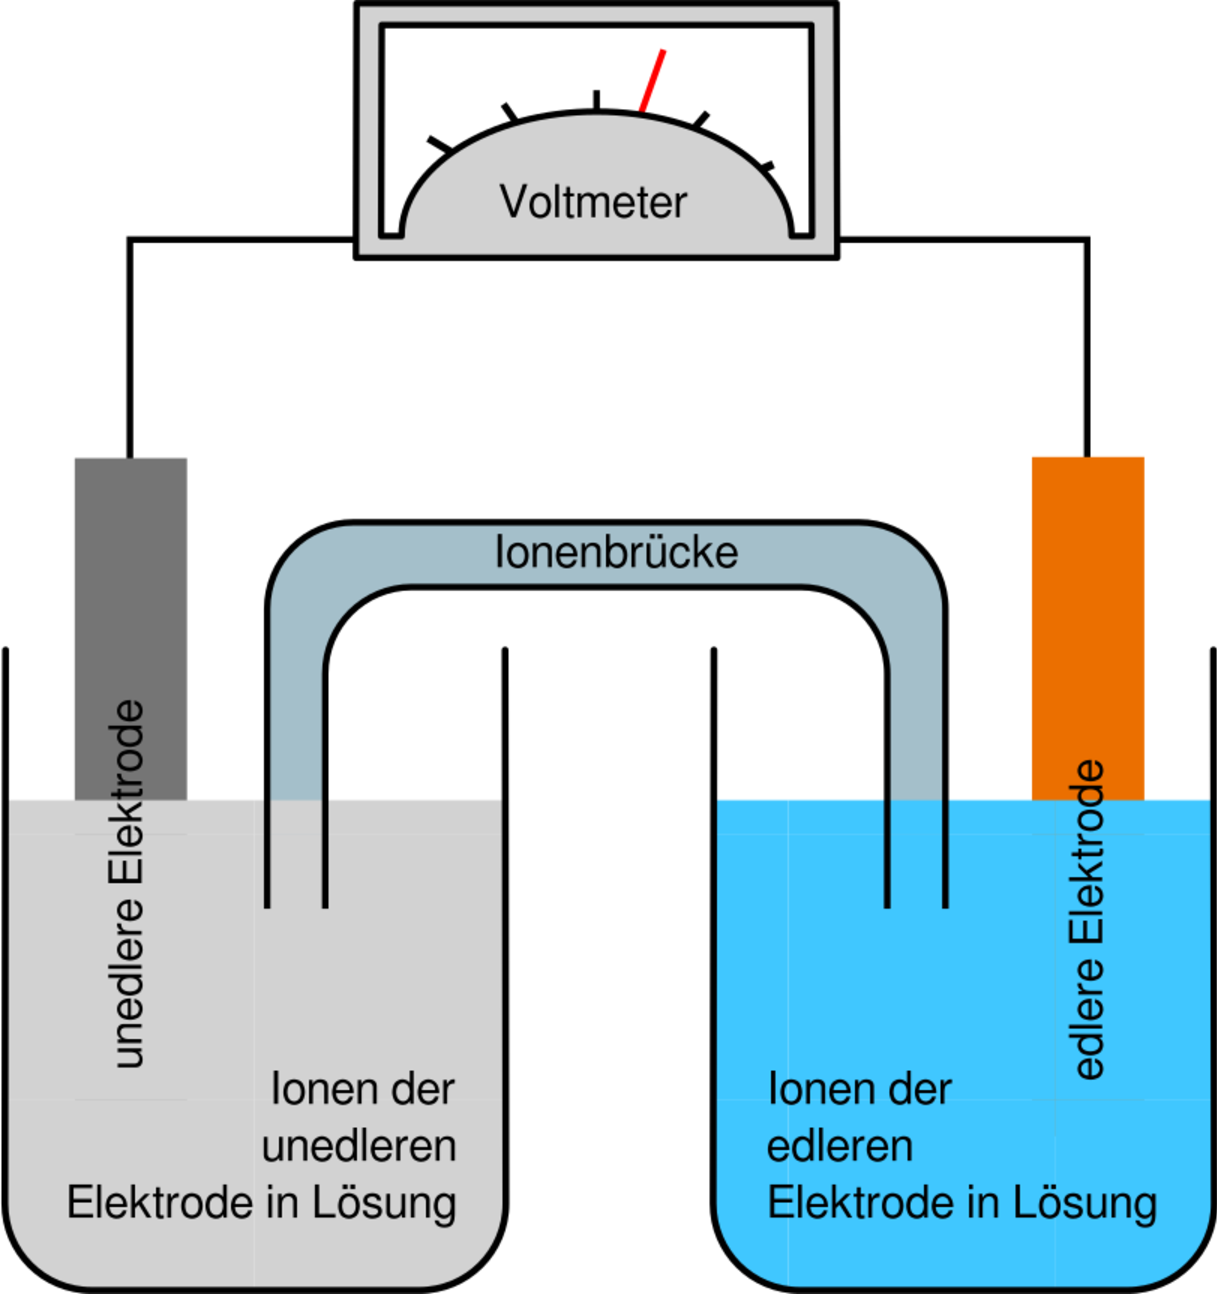
\includegraphics[width=0.8\textwidth]{Galvanische_Zelle.pdf}
		\subcaption{Galvanisches Element}
		\label{Galvanisches_Element}
	\end{subfigure}
	\begin{subfigure}{0.5\textwidth}
		\centering
		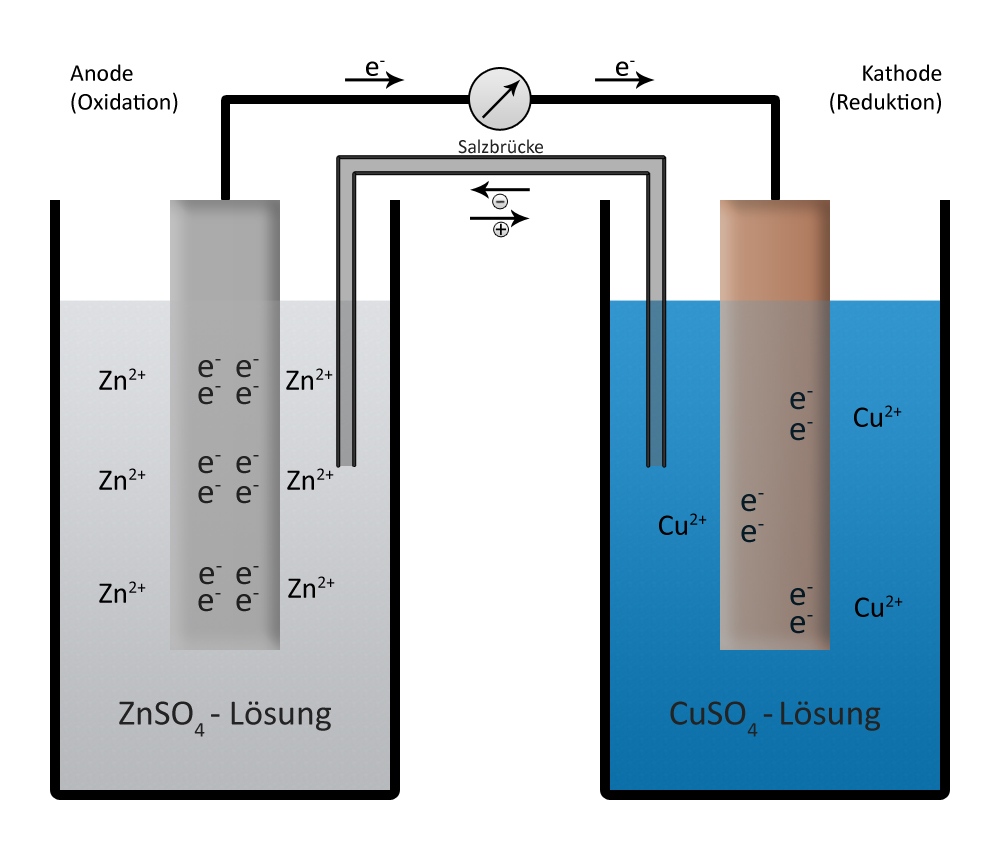
\includegraphics[width=\textwidth]{Daniell-Element.jpg}
		\subcaption{Daniell Element}
		\label{Daniell_Element}
	\end{subfigure}
\end{figure}
In jedem der beiden Behälter befindet sich eine Elektrode (ein Elektronenleiter) in einem Elektrolyt (eine Flüssigkeit, die Ionen enthält). Beim Daniell-Element sind das beispielsweise ein Zinkstab in verdünnter Schwefelsäure und ein Kupferstab in Kupfersulfatlösung (siehe Abbildung \ref{Daniell_Element}).
Zink ist \glqq unedler\grqq\ als Kupfer, sodass am Zinkstab verhältnismäßig mehr Ionen in Lösung gehen. Der Zinkstab erhält dadurch einen höheren negativen Ladungsüberschuss und wird zum negativen Pol, also der Anode. Um diesen Ladungsüberschuss auszugleichen, wandern negative Ladungen über einen Stromkreis (in Abbildung \ref{Galvanisches_Element} das Voltmeter) zur Kathode, dem Kupferstab. Dort nehmen die gelösten Kupfer-Kationen die überschüssigen Elektronen auf und lagern sich am Kupferstab ab. Das ist ein Reduktionsvorgang
\[\ce{Cu^{2+} + 2e^- \rightarrow  Cu} \ ,\]
der mit der Oxidation am Zinkstab
\[\ce{Zn \rightarrow Zn^{2+} + 2e^-}\]
einhergeht.
Gleichzeitig bekommt die Zinksulfatlösung einen immer höheren positiven Ladungsüberschuss, da ständig neue Zink-Kationen ausgelöst werden. Um das auszugleichen fließen Zink-Kationen über die Ionen-Brücke zur Kathode (der Halbzelle mit dem Kupferstab und der Kupfersulfatlösung) und Sulfat-Anionen \ce{[SO_4]^{2-}} in die entgegengesetzte Richtung zur Anode. \\
Dieser Ionenfluss geht nicht ohne \glqq Reibung\grqq\ aufgrund von elektrostatischen Wechselwirkungen von statten. Daher kommt der Innenwiderstand.

\subsubsection{RC-Generator}

\subsection{Messinstrumente}


\subsection{Widerstände}
